\subsection{Beam Quality}

As described in section xx, we have several beam counters to indentify beam particles event by event(see Fig\ref{fig:Beamline}).Using this when taking data, we can get data of interest selectively.The following describe how to identify beam particles with the typical data (Data Name:PhysicsOct48) including $K^{+}$, $\pi~{+}$, $e^{+}$, $p$ events, and their momentum adjusted $\sim$800MeV/c. \\

\begin{figure}[htbp]
  \centering
  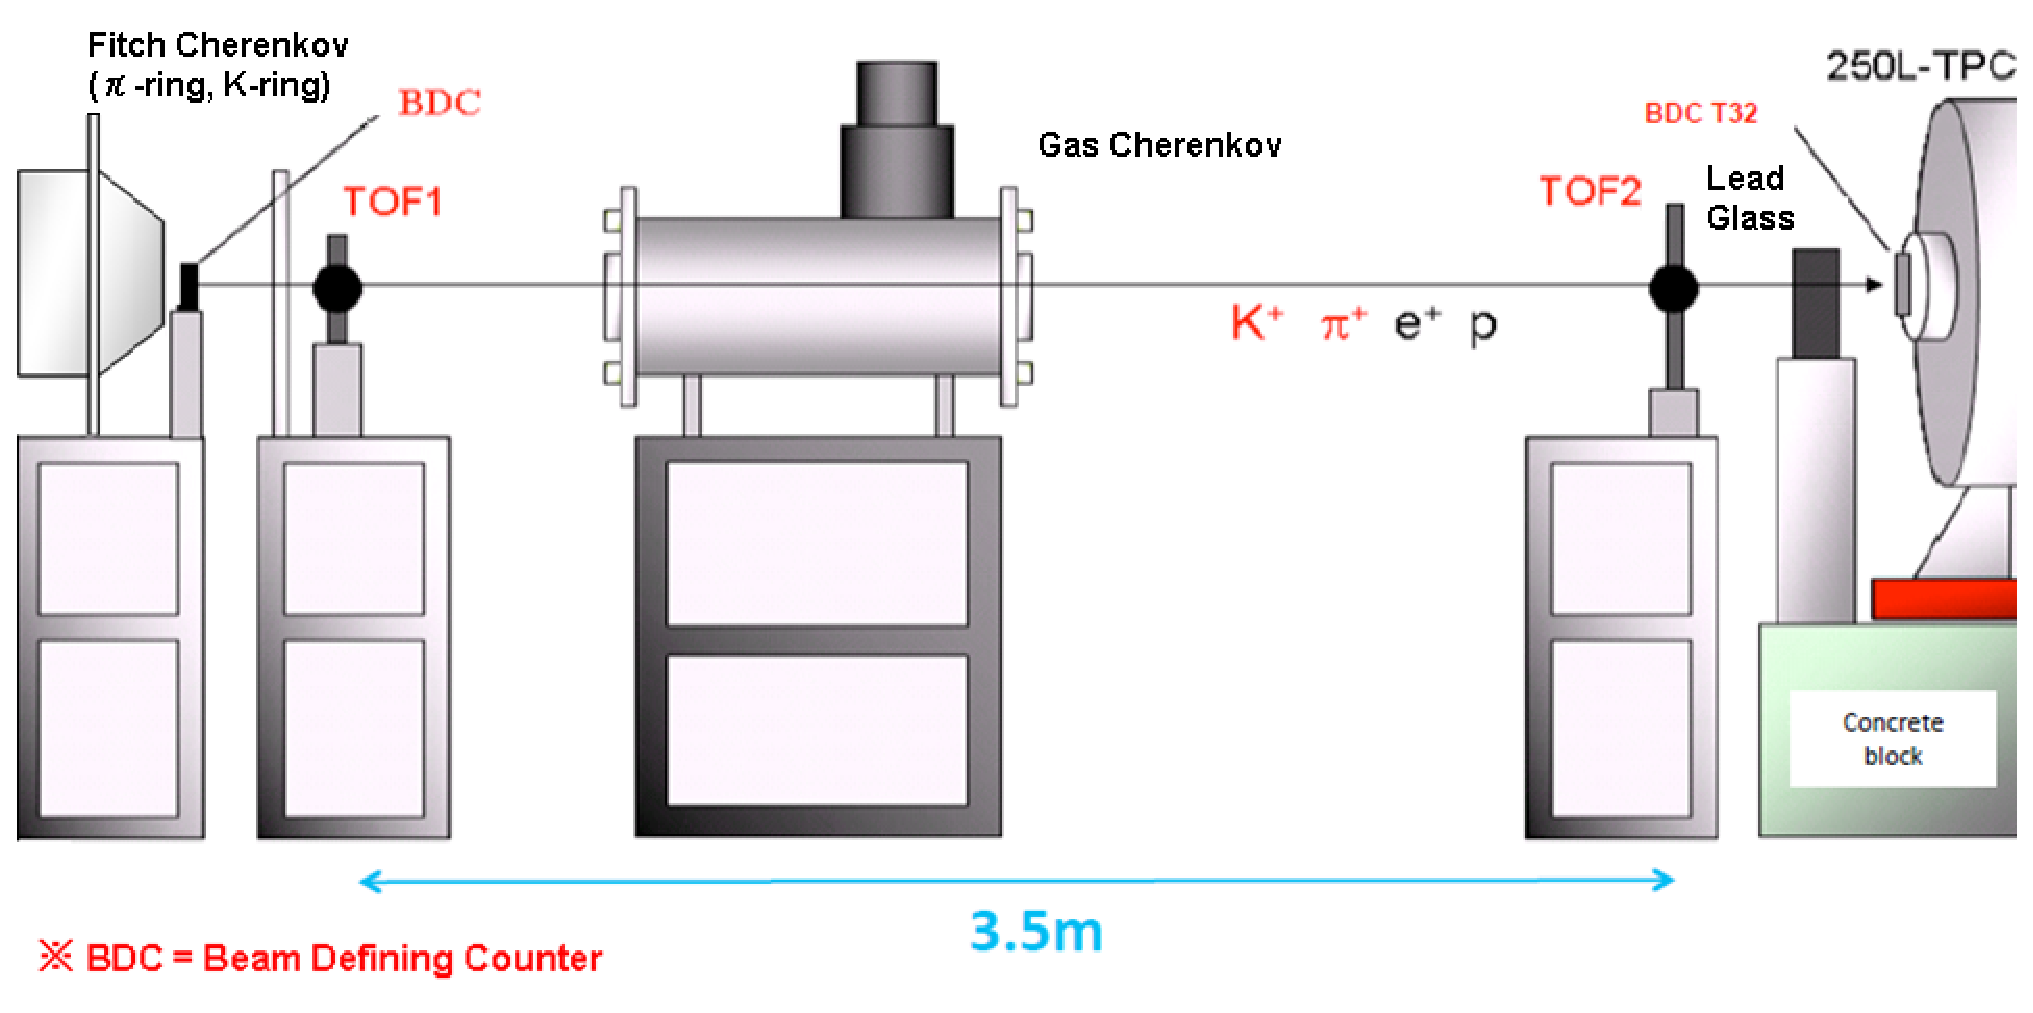
\includegraphics[width=10cm,clip]{fig/Beamline.eps}
  \caption{Instruments on K1.1BR Beam Line}
  \label{fig:Beamline}
\end{figure}

Leaded particles to K1.1BR beamline pass the Fitch Cheernkov Counter.
Fitch Cherenkov Counter can select particles with diffrerences of angle of cherenkov light which they radiate.
Fifure\ref{fig:FC_KPI} shows respose of the Fitch Cherenkov Counter.
The horizontal axis shows the total amount of PMT signal where cherenkov light of 800MeV/c $\pi$ can be detected.
The vertical axis shows that of 800MeV/c $K$.
Signal are distinctly seperated to three cluster and can be categolized as following.\\

\begin{enumerate}
\item FC Signal($\pi$)$<$1450 \& \& FC Signal($K$)$>$2000 \\
\item FC Signal($\pi$)$<$1450 \& \& FC Signal($K$)$<$2000 \\
\item FC Signal($\pi$)$>$1450 \& \& FC Signal($K$)$<$2000 \\
\end{enumerate}

Appearently, particles within the region 1 are $K^{+}$ candidates.
Particles within region 2 are $p$ candidates because 800MeV/c $p$ is impossible to radiate cherenkov light.
Particles within region 3 are $\pi^{+}$ or $e^{+}$ candidates because angle of cherenkov light are the same level.

\begin{figure}[htbp]
  \centering
  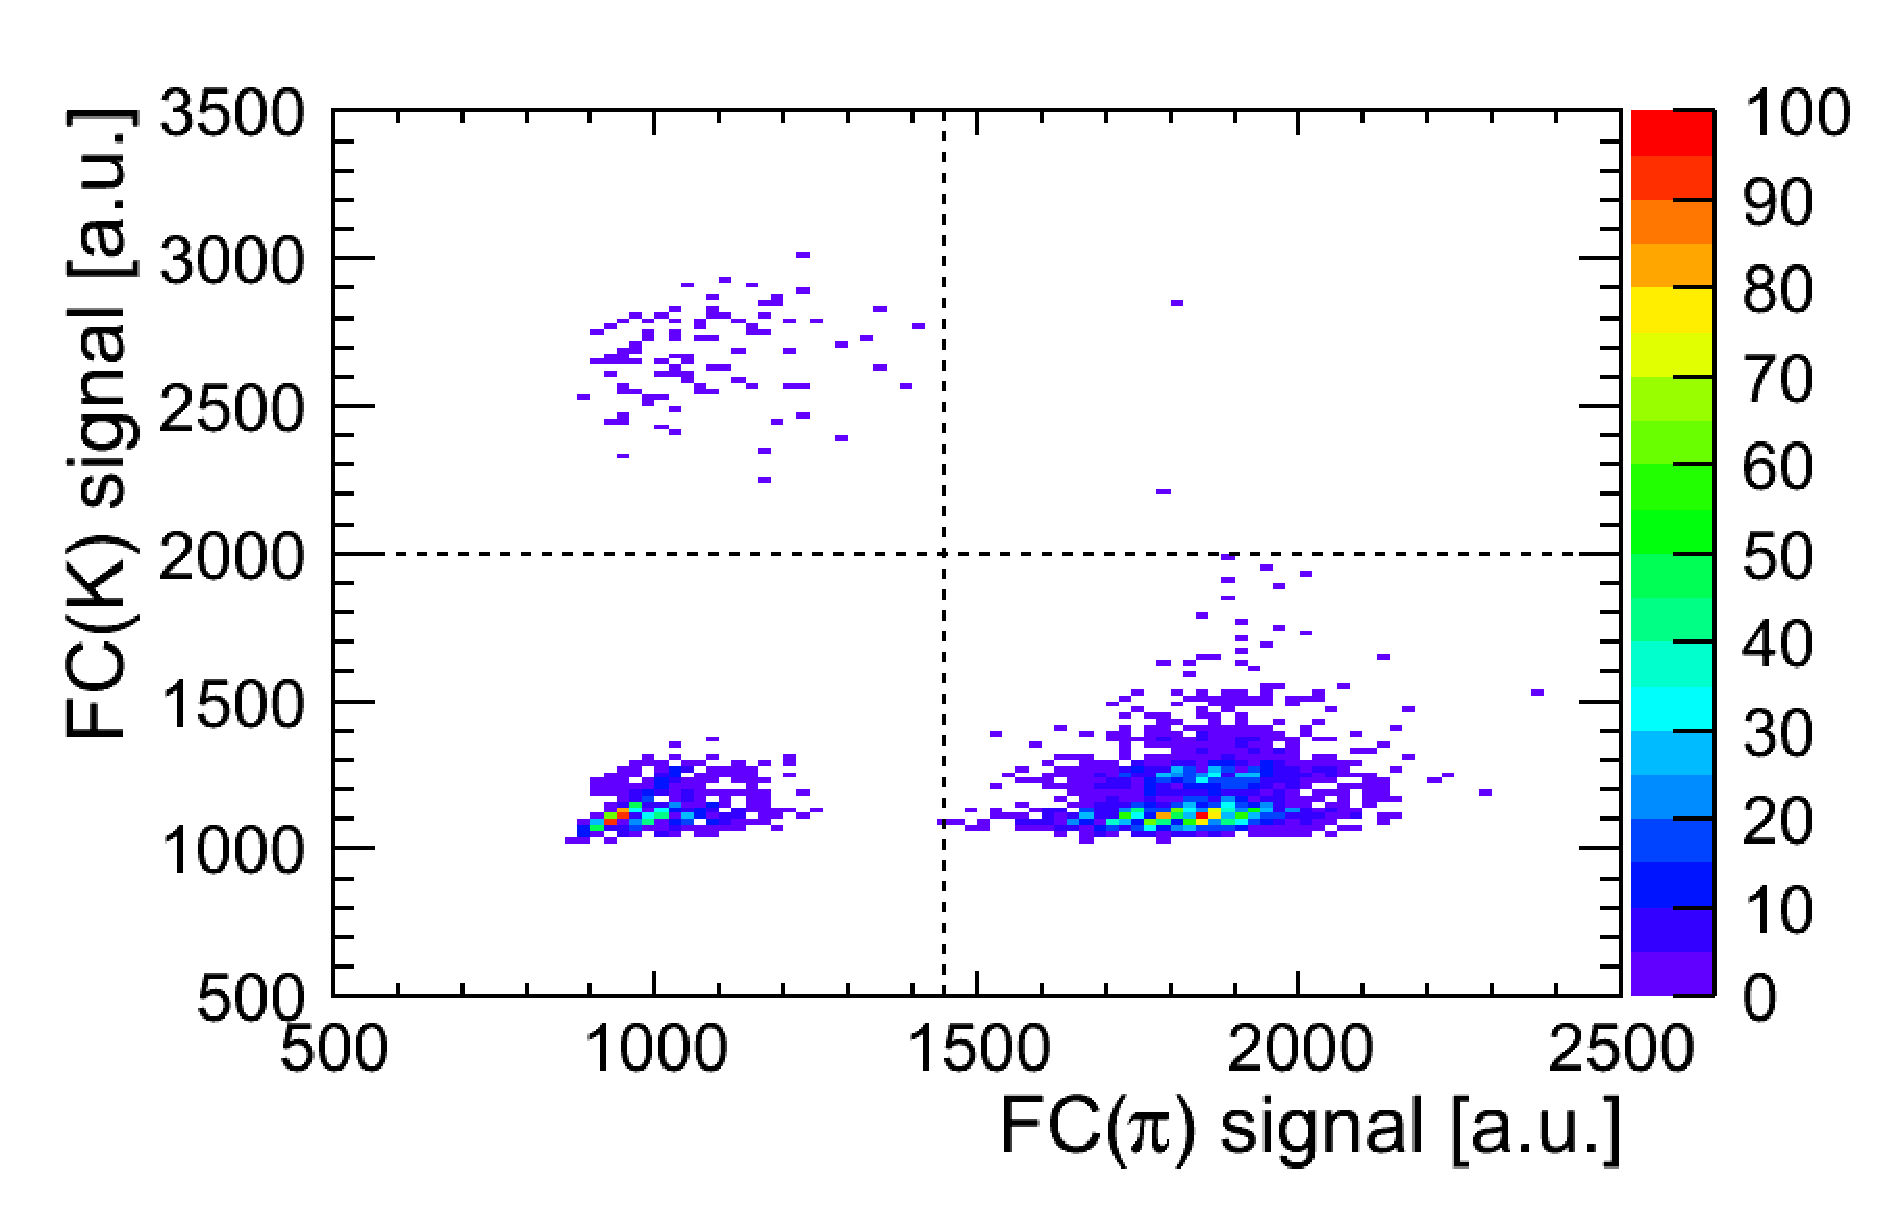
\includegraphics[width=10cm,clip]{fig/FC_KPI.eps}
  \caption{Fitch Cherenkov Counter}
  \label{fig:FC_KPI}
\end{figure}

Next, beam particles passed the TOF Counter.
There are two TOF Counters whose distance is 3.5m, 
and each particles can be separated with the difference of time of flight between them.
Following table\ref{tb:TOF_expect} is calcurated time of flight when each 800MeV/c particles passes two conters.\\

\begin{table}
  \centering
  \begin{tabular}[htb]{c|cccc}\hline
    particle & $e^{+}$ & $\pi^{+}$ & $K^{+}$ & $p$ \\ \hline
    Mass(MeV) & 0.511 & 139.57 & 493.68 & 938.27 \\
    Time of Flight($ns$) & 11.67 & 11.84 & 13.71 & 17.98 \\ \hline
  \end{tabular}
  \caption{Time of flight of eash particles}
  \label{tb:TOF_expect}
\end{table}

Figure\ref{fig:TOF} shows responce of the TOF Counters.
The horizontal axis shows the difference of time information between TOF1 and TOF2 Counter.
However, because the timing of zero of time infomation isn't matched between them, 
the horizontal axis are shifted paral from the real time of flight.
The vertical axis shows the number of events.
Signal have clearly divided structure and can be categolized as following.
From table\ref{tb:TOF_expect}, the region1 include $e^{+}$ or $\pi^{+}$ candidates,
and the region2 include $K^{+}$ candidates, and the region3 include $p$ candidates.\\

\begin{enumerate}
\item Time of Flight$<$the value added 4.5$\sigma$ to the mean of the left structure \\
\item above boundary value$<$Time of Flight$<$8.75(because of the clear separation from the right structure) \\
\item Time of Flight$>$8.75 \\
\end{enumerate}

\begin{figure}[htbp]
  \centering
  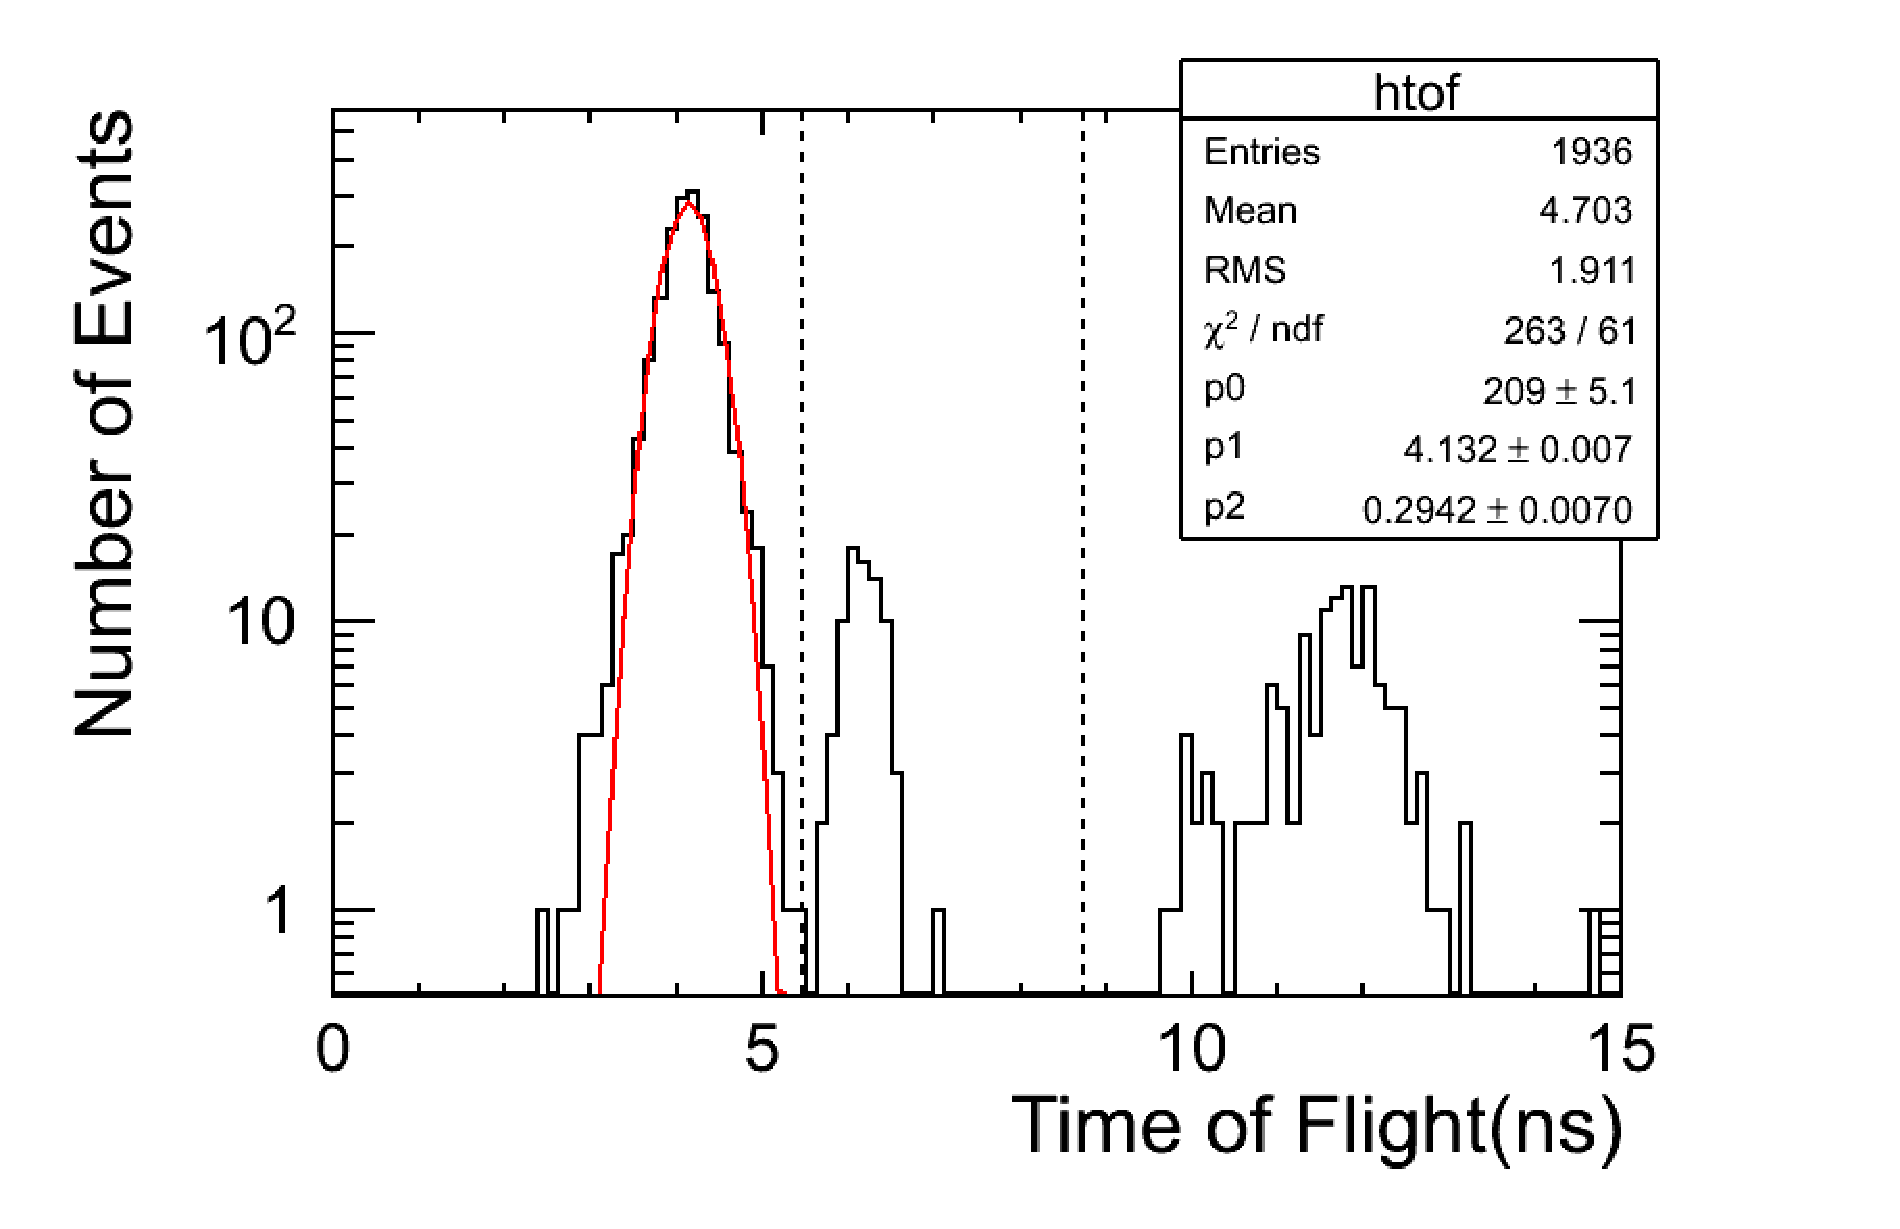
\includegraphics[width=10cm,clip]{fig/TOF.eps}
  \caption{TOF Counter}
  \label{fig:TOF}
\end{figure}

Fitch Cherenkov Counter and TOF Counter can't identify $e^{+}$ and $\pi{+}$.
However, Gas Cherenkov Counter can detect $e^{+}$ because the gas in this detector has the refractive index
only $e^{+}$ can radiate cherenkov light.
Figure\ref{fig:GC} shows responce of the Gas Cherenkov Counter.
The horizontal axis shows the PMT signal of Gas Cherenkov Counter.
Fitting the pedestal with gaussian,
the events larger by the value added 3.5$\sigma$ to the mean of the pedestal is $e^{+}$ candidates.\\

\begin{figure}[htbp]
  \centering
  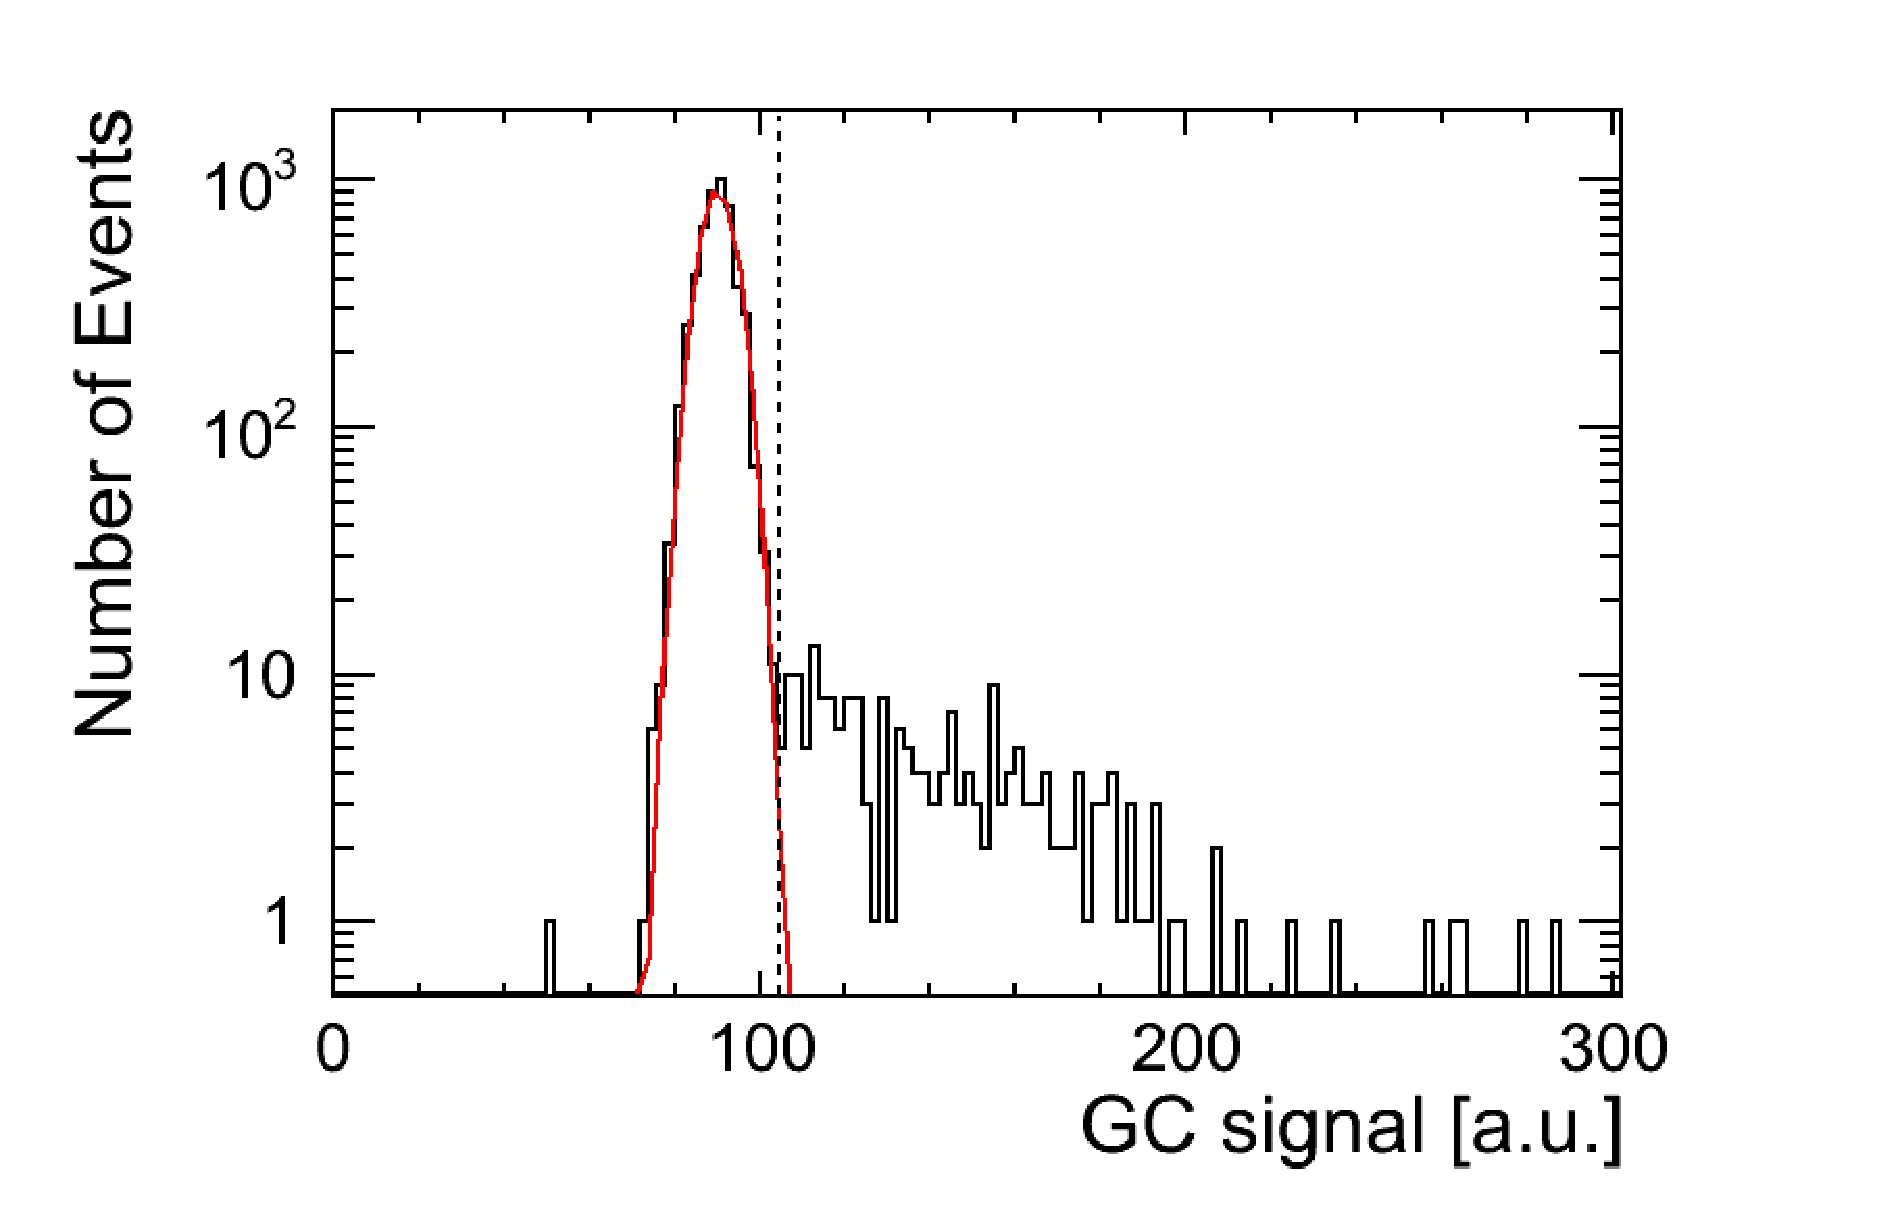
\includegraphics[width=10cm,clip]{fig/GC.eps}
  \caption{Gas Cherenkov Counter}
  \label{fig:GC}
\end{figure}

Particles which satisfy all conditions for the same candidate are identified them,
and the others are defined `uncertain` particles.
Herewith, we can identify beam particles with high purity before injection to 250L detector.
Table\ref{tb:component} shows the beam components of the data used for analysis.
It should be noted that the values used categolization are changed as appropriate.\\

\begin{table}
  \centering
  \begin{tabular}[htb]{ccccccc}\hline
    Data Name    & $e^{+}$ & $\pi^{+}$ & $K^{+}$ & $p$   & $uncertain$ & Number of Events \\ \hline
    PhysicsOct42 & 68      & 1617      & 27      & 232   & 5           & 1949             \\
    PhysicsOct48 & 128     & 1594      & 78      & 126   & 11          & 1937             \\
    PhysicsOct49 & 0       & 341       & 0       & 1146  & 12          & 1499             \\
    PhysicsOct52 & 0       & 1         & 3126    & 0     & 76          & 3203             \\
    PhysicsOct55 & 0       & 6         & 8386    & 0     & 208         & 8600             \\
    PhysicsOct59 & 0       & 8         & 5863    & 0     & 119         & 5963             \\
    PhysicsOct60 & 0       & 1         & 1870    & 0     & 40          & 1911             \\ \hline
  \end{tabular}
  \label{tb:component}
  \caption{Beam components of data ued for analysis}
\end{table}

PhysicsOct52,55,59,60 is the data which was required `FC signal($K$)$<$2000` when taking data for analysis.
As table\ref{tb:component} shows, these data is almost occupied $K^{+}$ events and the ratio is $\sim$98\% on average.